\subsection{Overall Framework}
\label{sec:overall}

We propose SynGS, a sparse-view 3D Gaussian Splatting framework that integrates explicit geometry initialization, depth-guided densification, and visibility-aware optimization. As illustrated in Fig.~\ref{fig:framework}, the input consists of sparse-view images and corresponding foreground masks, and the output is an optimized 3D Gaussian representation.

% Placeholder — replace path when the figure is ready
% \begin{figure}[ht]
% \centering
% 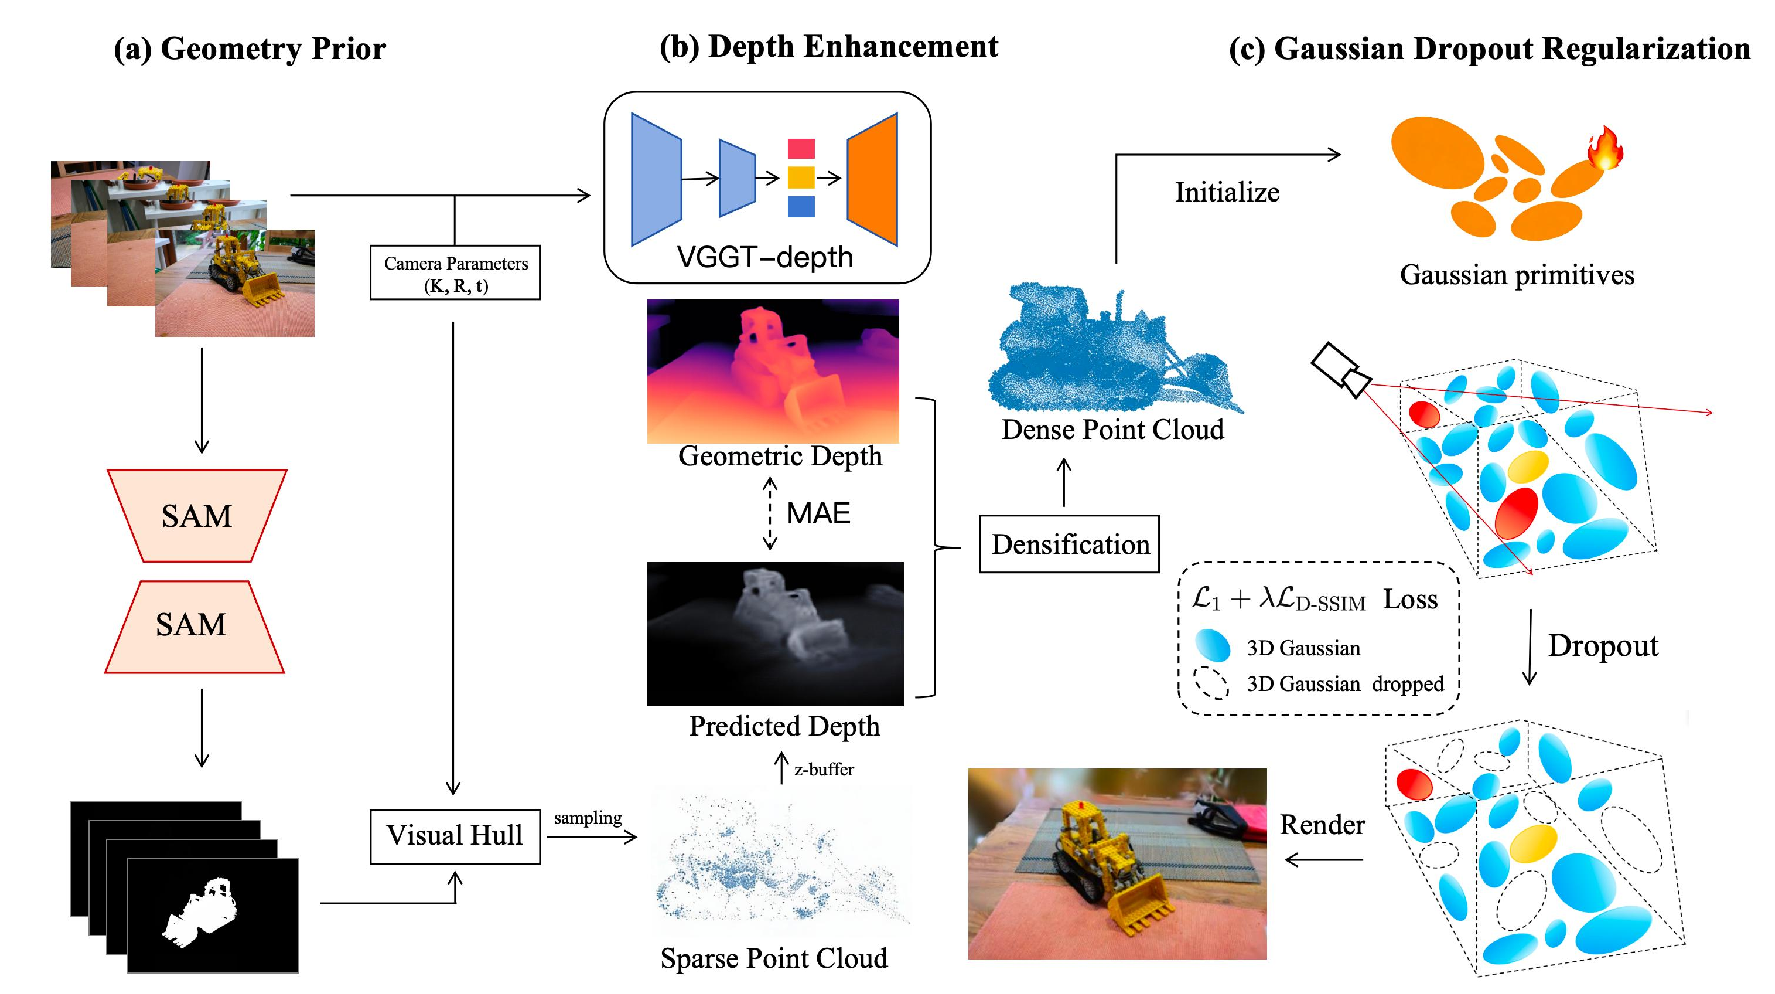
\includegraphics[width=\textwidth]{figures/framework.pdf}
% \caption{Overview of the SynGS pipeline. The third stage applies Dynamic Visibility Regularization (DVR).}
% \label{fig:framework}
% \end{figure}

The pipeline contains three consecutive stages. First, \textbf{Visual Hull Initialization} constructs a coarse geometric prior from multi-view silhouettes and generates an initial point cloud. Then, \textbf{VGGT / Depth-Guided Densification} exploits cross-view depth priors to supplement missing geometry and produce a depth-enhanced point cloud for Gaussian initialization. Finally, \textbf{Dynamic Visibility Regularization (DVR)} is applied during 3DGS optimization to rebalance supervision under sparse visibility and reduce overfitting artifacts. The complete process follows the pipeline:
\begin{equation}
\label{eq:pipeline}
\text{Visual Hull point cloud}
\rightarrow
\text{depth-enhanced point cloud}
\rightarrow
\text{Gaussian initialization}
\rightarrow
\text{DVR-regularized 3DGS optimization}.
\end{equation}
